\section{Frequency mode 01}
\label{FM01}

\subsection{Spectra}
\label{FM01:spectra}

\begin{figure}[ht]
    \centering
    \begin{subfigure}[b]{0.9545\textwidth}
        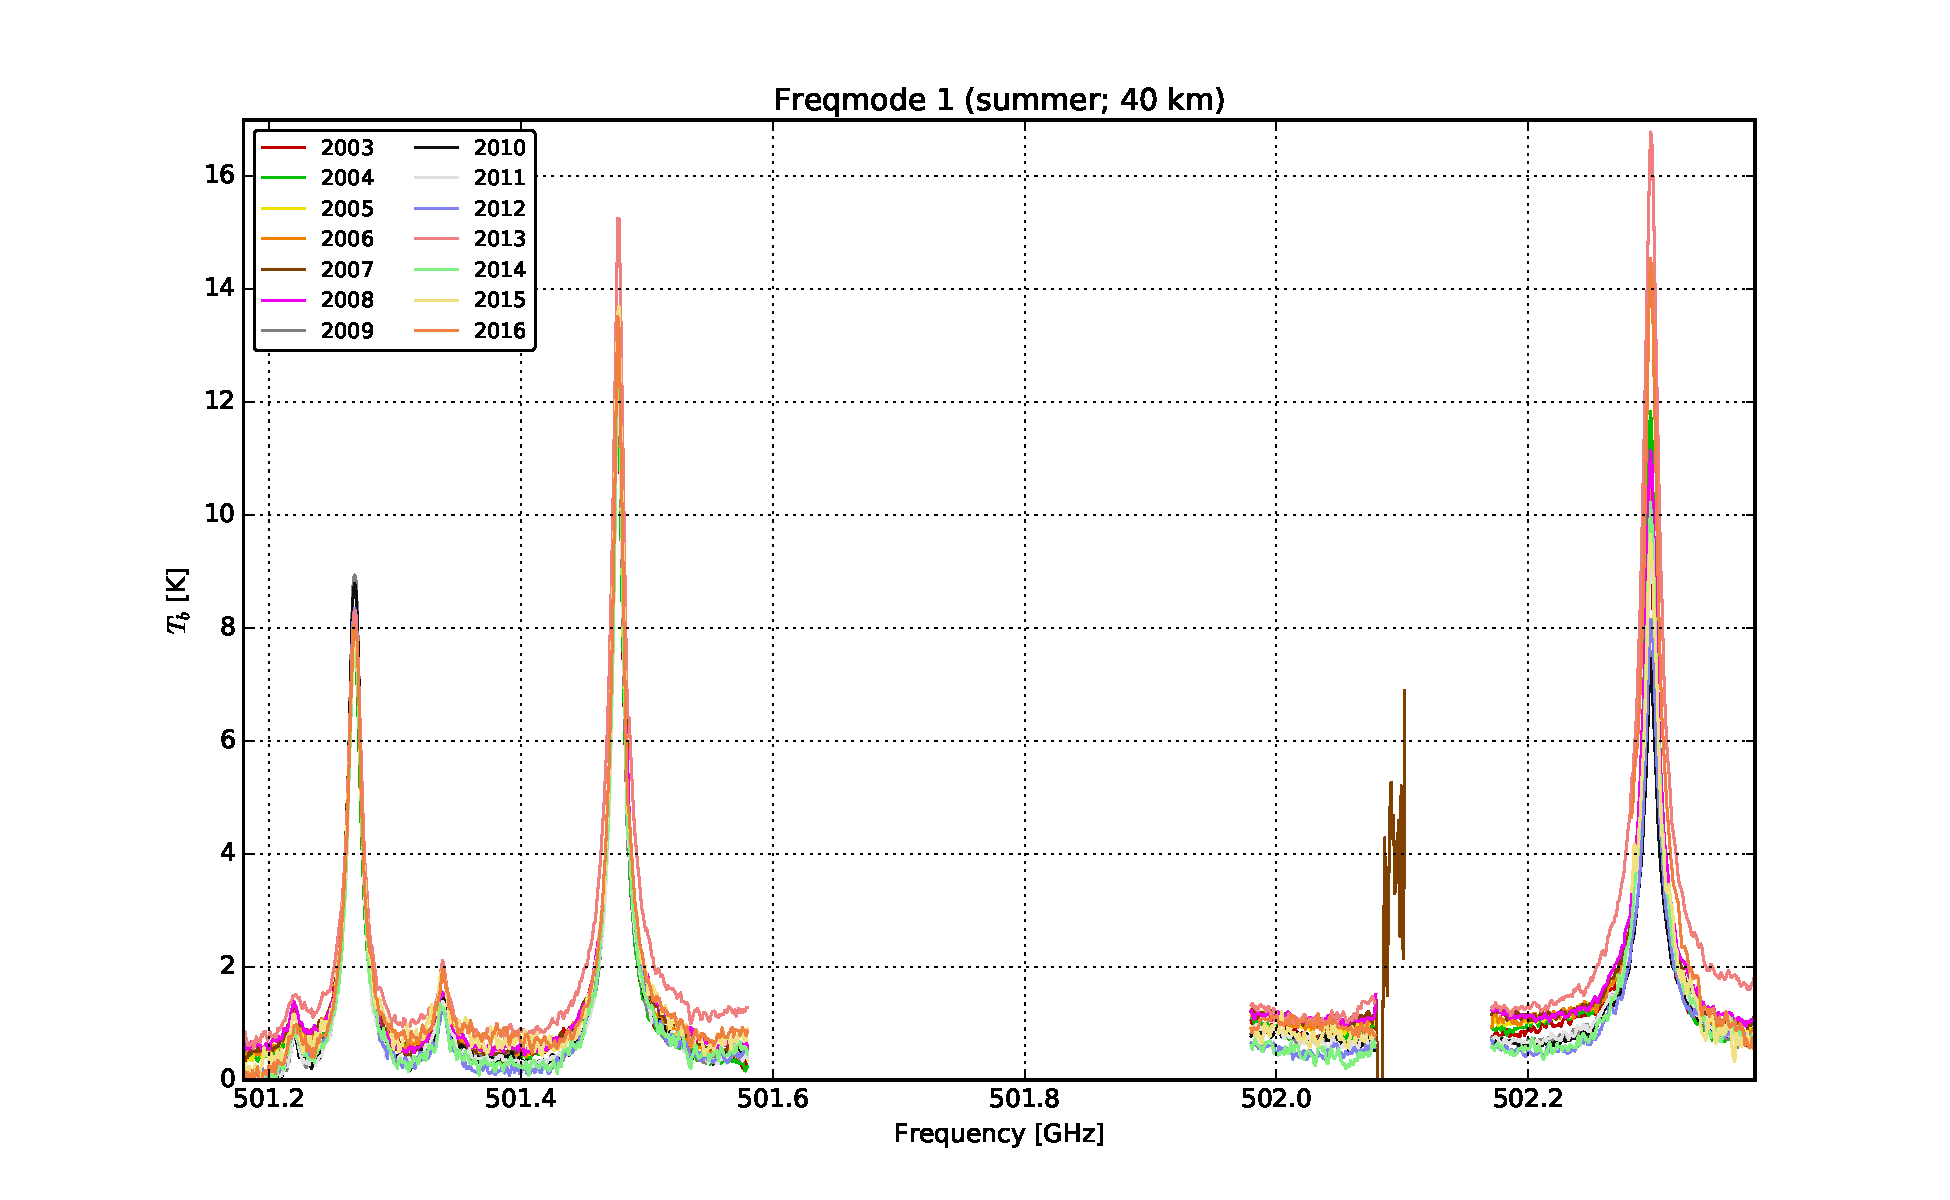
\includegraphics[width=\textwidth]{fm_01_spectra_summer}
        \caption{summer}\label{fig:spectra:01:summer}
    \end{subfigure}
    \begin{subfigure}[b]{0.9545\textwidth}
        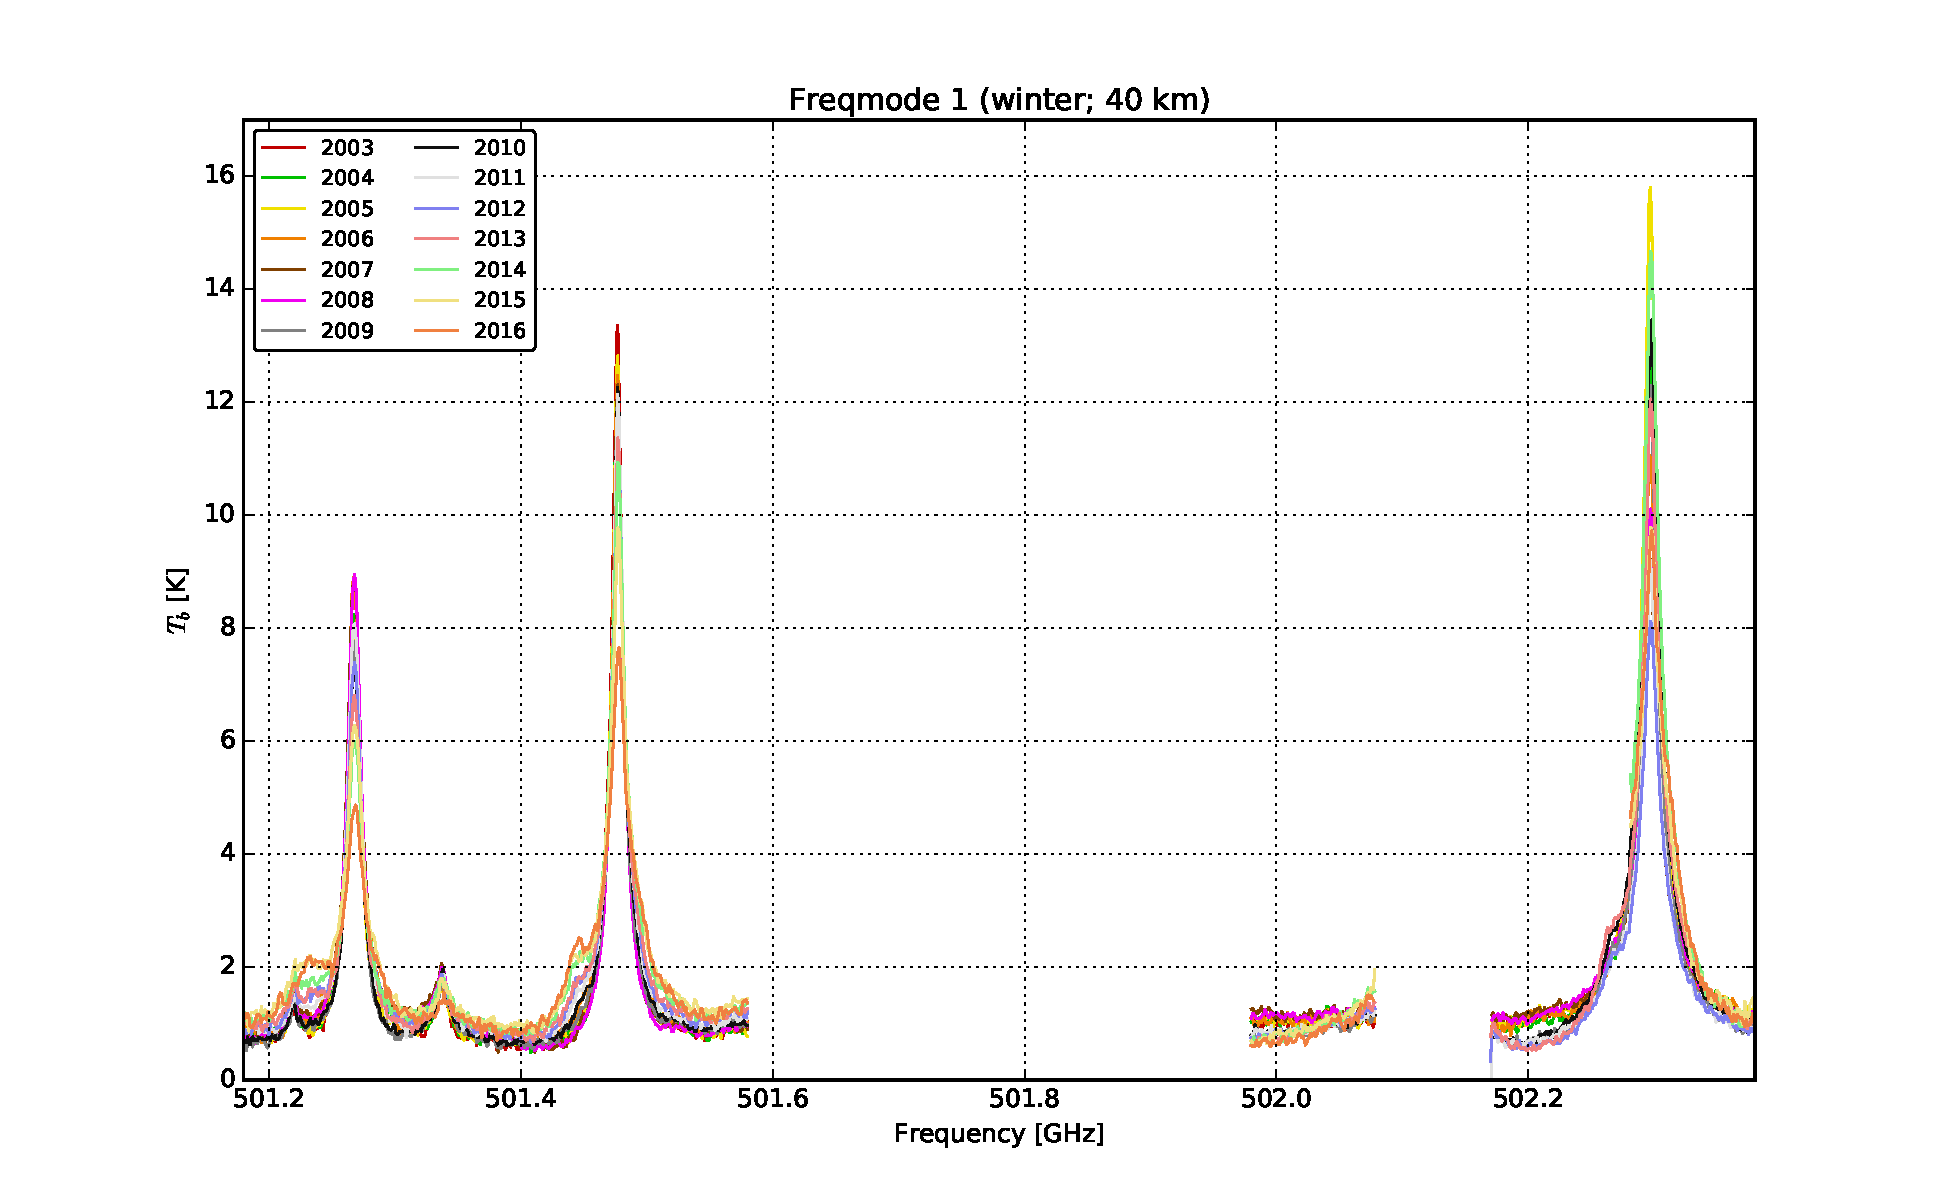
\includegraphics[width=\textwidth]{fm_01_spectra_winter}
        \caption{winter}\label{fig:spectra:01:winter}
    \end{subfigure}
    \caption{Annual median spectra for FM~01 for altitude interval 35--45~km at
        equatorial latitudes. The unhealthy sub-bands~3 and~7 are between
        $\sim502.08$ and~$502.28\,\mathrm{GHz}$.
        }\label{fig:spectra:01}
\end{figure}

\begin{figure}[ht]
    \centering
    \begin{subfigure}[b]{0.9545\textwidth}
        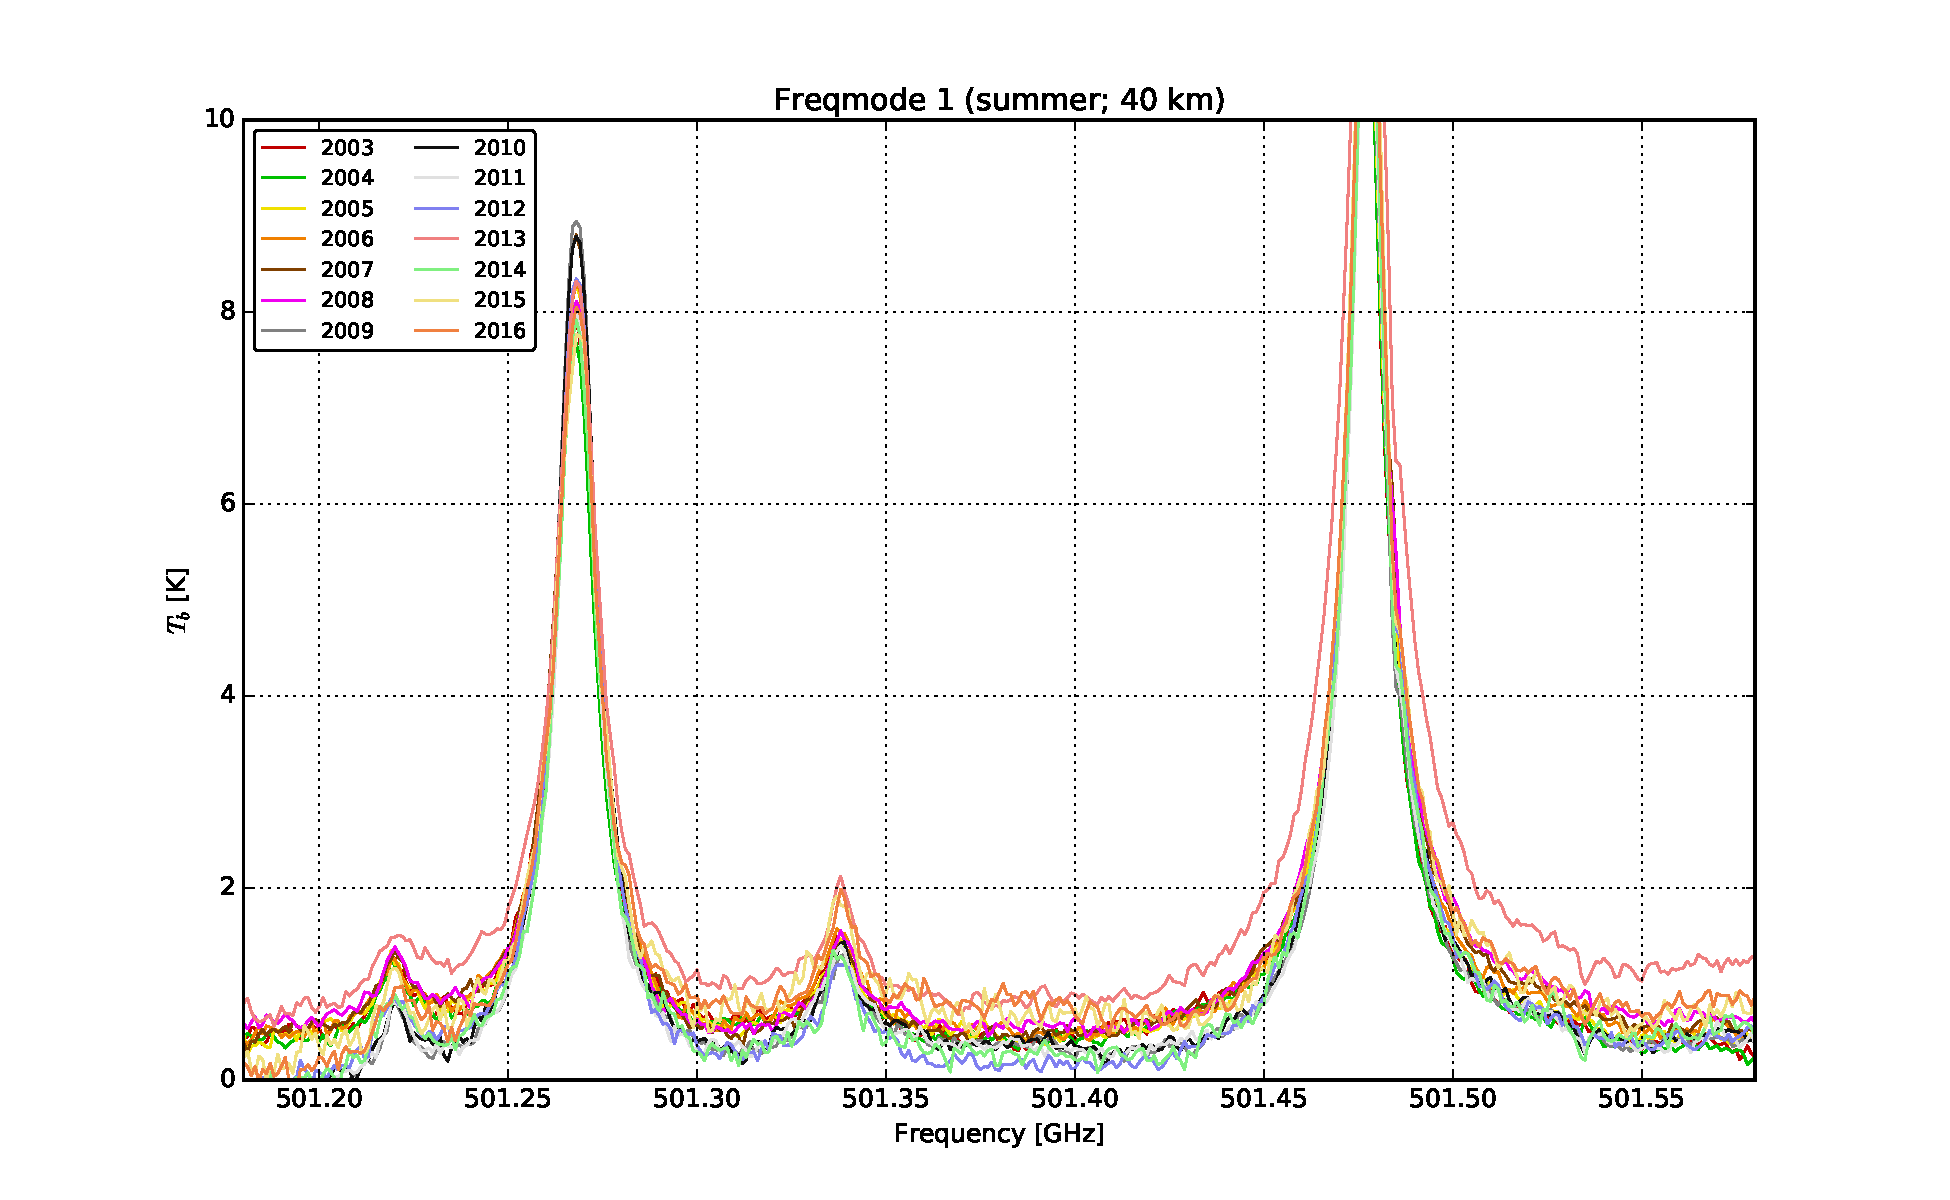
\includegraphics[width=\textwidth]{fm_01_spectra_summer_zoom_40km}
        \caption{summer}\label{fig:spectra:01:summer:closeup}
    \end{subfigure}
    \begin{subfigure}[b]{0.9545\textwidth}
        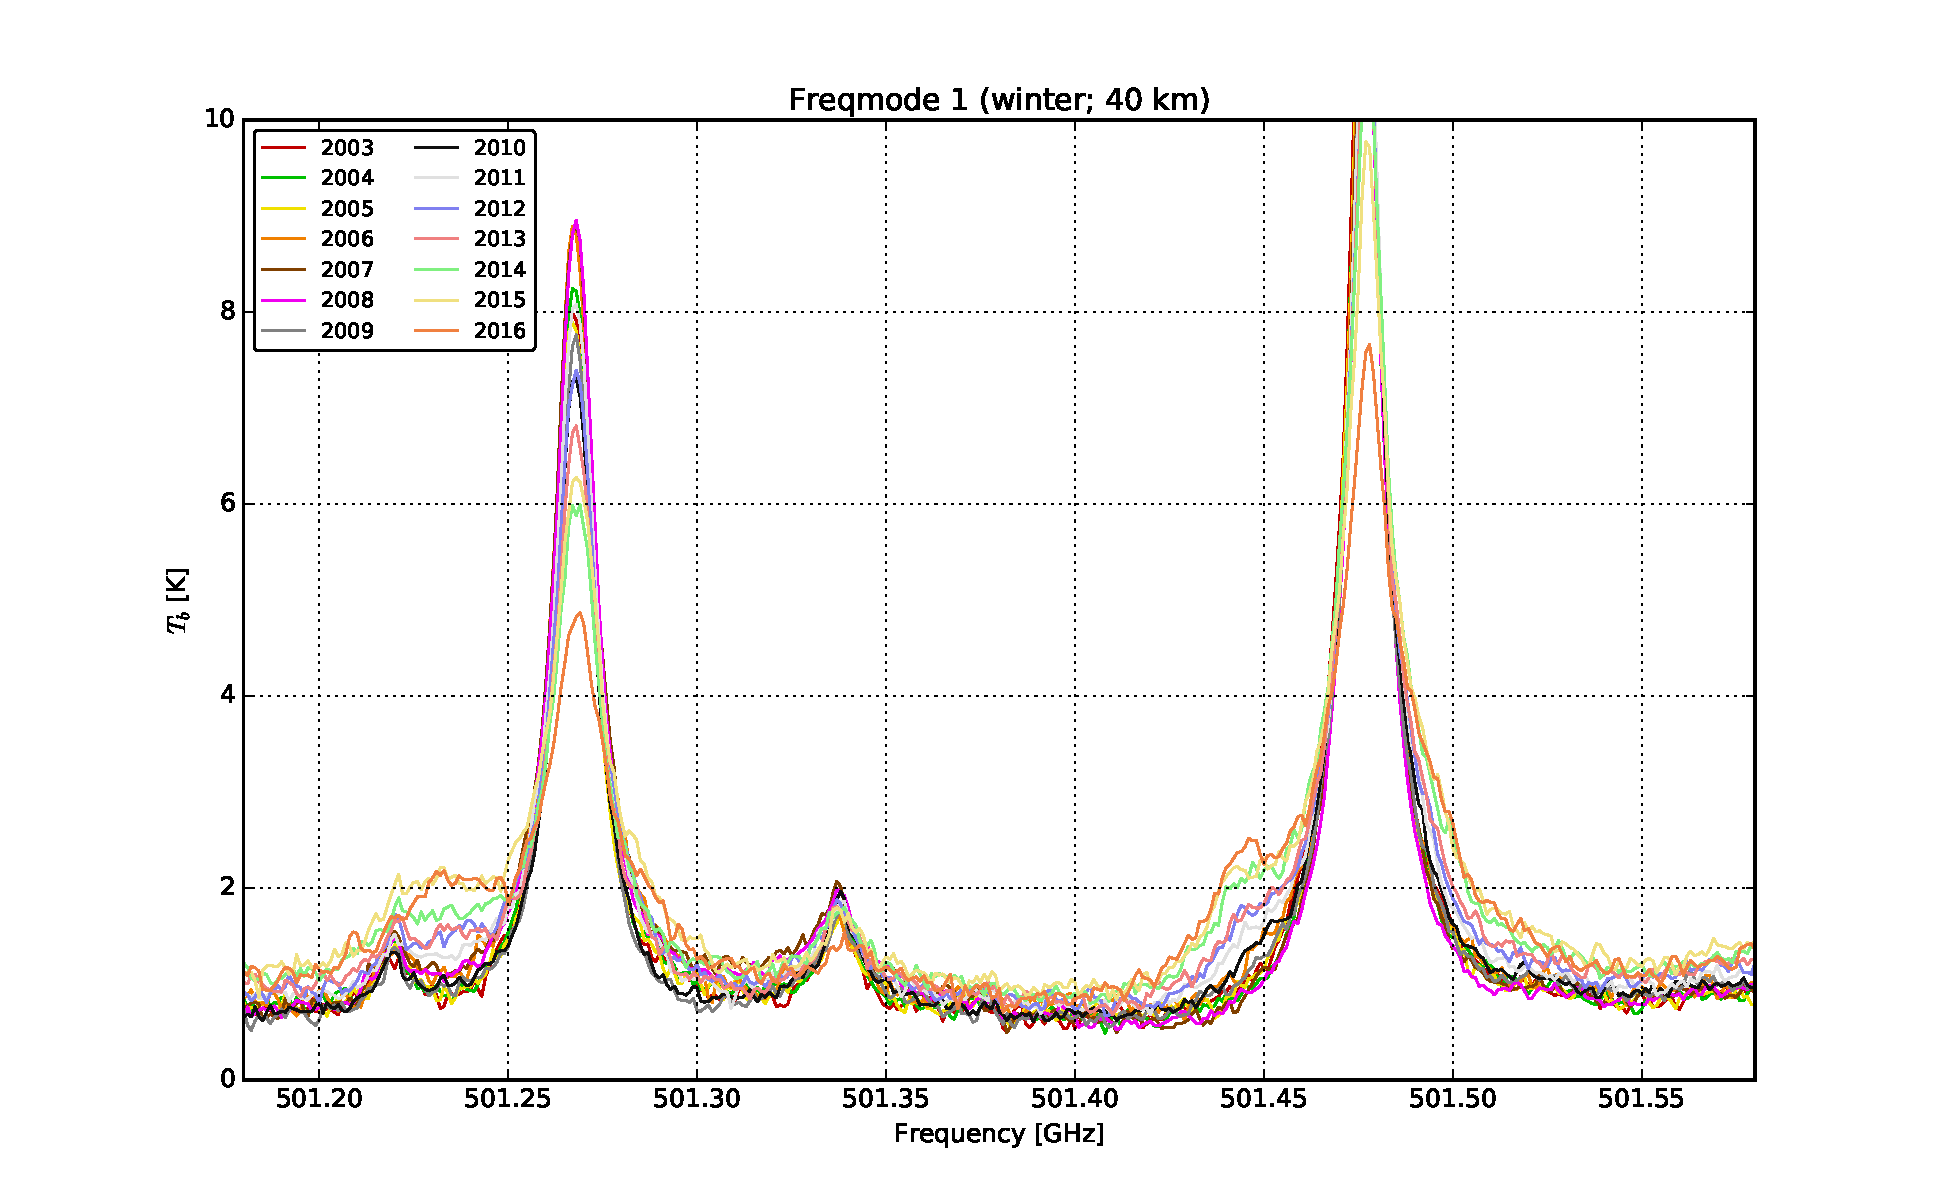
\includegraphics[width=\textwidth]{fm_01_spectra_winter_zoom_40km}
        \caption{winter}\label{fig:spectra:01:winter:closeup}
    \end{subfigure}
    \caption{Close-up of the annual median spectra for FM~01 for altitude
        interval 35--45~km at equatorial latitudes.
        }\label{fig:spectra:01:closeup}
\end{figure}

\noindent
Yearly median spectra for summer and winter at $\sim40\,\mathrm{km}$ are shown
\TODO{write up about FM1 spectra in general}


\subsection{Sideband leakage}
\label{FM01:sbl}
In FM~1 there are two sideband peaks to the right of the main band peak at
$503.3\,\mathrm{GHz}$, but these are note distinct in the spectra show in
Fig.~\ref{fig:spectra:01}.  Furthermore, the fact that these peaks are close
together near the edge of the spectra makes it difficult to extract an
approximate mainband baseline to subtract from the peaks such as they are.  It
is therefore very difficult to draw any conclusions as to the long term trends
of the sideband leakage for this mode, but a rough very rough estimate would be
$\sim3$--$7$\%.  A slight tendency to increase over time can be discerned if
one looks closely and squints, but this may be attributed to confirmation bias
on the part of the investigator and should be regarded as speculation at this
point.


\subsection{Seasonality}
\label{FM01:seasonality}
\TODO{New peak figure}
\TODO{Left-wings}

\subsection{Change of ``base line'' for later years}
\label{FM01:baseline}
\TODO{New peak figure (same as above)}
\TODO{Baseline left of \chem{N_2O}}

\subsection{Left-wing splitters}
\label{FM01:leftwings}
\TODO{intro}
From Fig.~\ref{fig:spectra:01:closeup} it is clear that the effect assymetric
and therefore not a simple broadening of the lines.
Rather it appears that spectral intensity has been moved from the peak values
and deposited over an interval $\sim50\,\mathrm{MHz}$ beginning below the peak.
Since the figure shows median spectra, this is consistent with a portion of
spectra having been shifted to to lower frequencies, misplacing the peak.  So
far this hypothesis has not been confirmed whehn looking at individual spectra,
but it should be more thoroughly investigated before being ruled out.  One
route ahead might be to look at daily spectra, though if the phenomenon is
similar to that of the \chem{CO} modes (FMs~14, 22 and~24) the shift likely
occurs during the beginning of a measurement period, which might make it hard
to spot using this method.

As noted above and seen in Fig.~\ref{fig:spectra:01:closeup}, the phenomenon is
only evident during the winter, which indicates that it might be temperature
dependent since during the winter the satellite is warmer (see~\ref{sec:Tcal}).

As seen in Fig.~\ref{fig:spectra:01}, the wings are not as evident around the
\chem{N_2O} at $\sim502.3\,\mathrm{GHz}$, which is likely due in part to the
afflicted region being in the unhealthy subband~7, which is missing from later
years.  Looking at the three main peaks in Fig.~\ref{fig:spectra:01:winter},
however, it appears that the ``shift'' may be more pronounced for lower
frequencies, with the left-most \chem{ClO}-peak showing the largest down-shift
and the right-most \chem{N_2O}-peak showing the smallest.  This frequency
dependence of the effect is speculative at this point, but might deserve
further investigation.  \TODO{Put numbers on shift?}
